\documentclass[11pt]{article}
\usepackage[margin=1in]{geometry}
\usepackage{amsmath, amssymb, amsthm}
\usepackage{graphicx}
\usepackage{xcolor}
\usepackage{hyperref}
\usepackage{algorithm}
\usepackage{algpseudocode}
\usepackage{setspace}
\usepackage{biblatex}
\usepackage{arydshln}
\setstretch{1.15}
\addbibresource{references.bib} %Import the bibliography file

\title{\textbf{SEARCH 22.5: Spectral Embedding Archive for Rational Crease Pattern Hyperspace}}
\author{Brandon Wong}
\date{\today}

\begin{document}

\maketitle

\begin{abstract}
This report presents SEARCH (Spectral Embedding Archive for Rational Crease Pattern Hyperspace), an inverted design methodology for computational generation of 22.5$^\circ$ crease patterns. Instead of solving a highly intractible nonlinear mixed-integer optimization problem for every user input, we precompute a massive database of millions of valid uniaxial 22.5$^\circ$ crease patterns. At runtime, the system then searches the database for the precomputed crease pattern whose uniaxial tree most closely matches the user's desired structure. The database uses laplacian eigenvalues of the uniaxial trees as embeddings to index structural similarity (\textit{spectral embedding archive}). Furthermore, floating point errors due to 22.5's inherent $\sqrt{2}$ computations are circumvented by projecting vertices onto a 4D rational basis (\textit{rational crease pattern hyperspace}). By shifting the computational burden to an exhaustive precomputation phase, user design is reduced to a FAISS query, which runs in constant time relative to input complexity. This report details the mathematical architecture of the database generation pipeline, which is divided into three phases: (I) Topology Enumeration, (II) Tiling optimization for foldability, and (III) Crease Pattern generation and tree extraction.


\end{abstract}

\section{Introduction}

One of the biggest unsolved problems in origami design is the ability to systematically design models in the 22.5$^\circ$ angle system, in which creases meet at angles of multiples of 22.5$^\circ$. Many of the oldest known traditional origami designs use this angle system (including the fish, crane, and frog), as do some of the most popular modern-day designs, yet there remain no known mathematical methods to systematically design models within these angle constraints. Instead, most 22.5$^\circ$ origami designers rely on trial and error combined with an experienced artist's intuition.

In general, representational origami designs can be categorized into two categories: uniaxial and non-uniaxial. Uniaxial designs are those whose structure can be represented by a tree of flaps and rivers. Forward design with uniaxial methods, including circle packing, box pleating, and hex pleating, have been well-studied. In these systematic procedures, a tree is converted into a packing of circles, squares, or hexagons by formulating the problem an optimization problem defined by non-linear non-intersection constraints. Then, a crease pattern can be obtained from the packing by linear time deterministic procedures

It is theoretically possible to inject rigid integer constraints into the nonlinear solver to enforce the angle constraints of the 22.5$^\circ$ system. However, even if this massive MINLP problem is solved and a valid packing is found, there is no known way to convert the packing into a flat foldable crease pattern due to a phenomenon known as ``dense bouncing''. Unlike box pleating or hex pleating with rational quantized lengths, 22.5$^\circ$ angles generate lengths involving $\sqrt{2}$, for which no amount of subdivision will ever perfectly line up with a rational length, effectively requiring an infinite number of creases to resolve the packing. And unlike circle packing which solves this by placing creases at specific angles, 22.5$^\circ$ crease patterns are by definition restricted to creases at multiples of 22.5$^\circ$. 

Conversely, generating a flat foldable crease pattern from a predefined tiling of 22.5$^\circ$ molecules is computationally straightforward through the use of straight skeletons. However, the inverse design of a tiling to acheive a desired tree has no known solution---in fact, prior to this project, there were no known implementations of the forward computation of extracting a tree from a tiling.

Therefore, we we exploit the computational tractibility of tilings to enumerate a massive database of valid 22.5$^\circ$ tilings, and then extract their underlying trees retroactively. By indexing the database using spectral embeddings of the uniaxial trees, we can approximate the user's inverse design problem (Tree $\to$ Crease Pattern) in constant time by simply searching for the closest spectral embedding in the database and returning its corresponding crease pattern.

\subsection{Packing, Tiling, and Molecules}

\subsection{Definitions and Nomenclature}
To document the SEARCH 22.5 data pipeline, we define the following levels of abstraction across our architecture:
\begin{itemize}
    \item \textbf{Topology:} An unweighted planar graph representing the angles (multiples of 45$^\circ$) and connective relationships of axial creases, prior to assigning specific lengths.
    \item \textbf{Tiling:} A metric realization of a topology, or in other words, a planar graph of axial creases with assigned lengths.
    \item \textbf{Crease Pattern:} A planar graph of creases that includes the axial creases of the tiling, ridge creases formed by the straight skeleton of the tiling polygons, and any additional creases (hinges) required to fold the model flat.
    % \item \textbf{Quadruplet:} A geometric configuration within a polygonal face where four boundary edges possess angular bisectors that converge at a single central point. 
    \item \textbf{Fold/Folded form:} The folded state of a crease pattern, defined by an unordered set of faces and their connectivity in 2d space. In this report, we neglect layer ordering and self intersection.
    \item \textbf{Uniaxial Tree:} The projection of the folded form onto some axis, resulting in a tree structure of flaps and rivers representing the stick figure of the folded form.
    % \item \textbf{Hypercube Basis:} A 4-dimensional algebraic basis in $\mathbb{Q}^4$ mapped to the Euclidean $\mathbb{R}^2$ plane. A vector $\vec{v} = [x, y, z, w]^T$ represents the physical 2D coordinate $\vec{p}$ via the mapping: $\vec{p} = x \vec{b}_1 + y \vec{b}_2 + z \vec{b}_3 + w \vec{b}_4$, where the basis vectors are $\vec{b}_1 = [1,0]^T$, $\vec{b}_2 = [s,s]^T$, $\vec{b}_3 = [0,1]^T$, and $\vec{b}_4 = [-s,s]^T$ with $s = \sqrt{2}/2$.
\end{itemize}

\section{Vertex and Crease Level Architecture}

The first major obstacle in the 22.5$^\circ$ system is representing vertices. In conventional crease pattern software, points are stored as floating-point Cartesian pairs. Because 22.5$^\circ$ triangles immediately generate irrational lengths, we encounter severe numerical precision issues during raycasting and intersection checking if we attempt to use this conventional data structure.

We observe that all Cartesian coordinates in the 22.5$^\circ$ angle system can be represented analytically in the form $(A_x + B_x\sqrt{2} , A_y + B_y\sqrt{2})$, where $A_x, B_x, A_y, B_y$ are rational numbers. This suggests that we can represent points as a tuple of four fractions, avoiding numerical drift entirely by storing the vertex as a list of integers.

\subsection{The 4D Hypercube Projection}
It would be possible to directly convert the 2D Cartesian coordinate to the orthogonal 4D rational coordinate $(A_x, B_x, A_y, B_y)$. However, we elect to use a projection that spaces the basis vectors 45 degrees apart from one another, reminiscent of projecting a 4D hypercube in 2D space. Rational 4D coordinates project uniquely to the 2D plane, and 2D 22.5$^\circ$ vertices ``lift'' uniquely into 4D. 

\textcolor{red}{[Figure Placeholder: A coordinate plane showing the 8-directional hypercube basis. The vertex (1,1,-1,1) is visually constructed by adding the basis vectors $\hat{x}, \hat{y}, -\hat{z}, \hat{w}$ tail-to-head.]}

\subsection{Crease Intersections and Exact Fractions}
To intersect creases formed by vertices $\vec{v}_a$ and $\vec{v}_b$ at angles $\alpha$ and $\beta$, we utilize precomputed rational tangents. The intersection vertex $\vec{v}_c$ is calculated as:
\begin{align}
    \Delta i & = (v_{b_x} - v_{a_x}) + (v_{b_y} - v_{a_y} - v_{b_w} + v_{a_w})\frac{\sqrt{2}}{2} \\
    \Delta j & = (v_{b_z} - v_{a_z}) + (v_{b_y} - v_{a_y} + v_{b_w} - v_{a_w})\frac{\sqrt{2}}{2} \\
    \beta_i & = \frac{\Delta j - \tan(\alpha)\Delta i}{\tan(\alpha) - \tan(\beta)}
\end{align}
To prevent exponential bit-depth growth during complex divisions, we implemented a custom, highly optimized C++ \texttt{Fraction} class exposed via Python bindings. This class strictly enforces immediate $\gcd$ simplification upon instantiation, ensuring the numerators and denominators remain safely within 64-bit integer limits across millions of operations.


% =================================
% =================================
% =================================


\section{Database Generation Phase I: Topology Enumeration}

To build an exhaustive database of 22.5$^\circ$ crease patterns, we must enumerate the valid arrangement of axial creases that define the tilings. A topology defines the angles and connective relationships of axial creases, disregarding exact metric lengths. We exhaustively enumerate every valid topology on an $N \times N$ integer grid by modeling the problem as a Boolean Satisfiability (SAT) problem.

\subsection{Grid Formulation and Boolean Variables}
We embed a planar graph onto an $N \times N$ square grid. The boundary of the paper is fixed, comprising $4N$ predefined boundary segments. 

Inside the grid, every possible orthogonal and diagonal segment connecting adjacent integer coordinates is treated as a potential axial crease. We assign a boolean decision variable $e \in \{0, 1\}$ to every internal edge.
% \begin{itemize}
%     \item \textbf{Orthogonal Edges:} Horizontal segments $e\_h_{i,j}$ connecting $(i, j)$ to $(i+1, j)$, and vertical segments $e\_v_{j,i}$ connecting $(j, i)$ to $(j, i+1)$.
%     \item \textbf{Diagonal Edges:} For every $1 \times 1$ cell with bottom-left coordinate $(x,y)$, two intersecting diagonals are defined: $d1_{x,y}$ connecting $(x,y)$ to $(x+1, y+1)$, and $d2_{x,y}$ connecting $(x+1,y)$ to $(x, y+1)$.
% \end{itemize}
The total number of internal boolean variables for an $N \times N$ grid is precisely $4N^2 - 2N$. The SAT solver's task is to sort through the $2^{4N^2 - 2N}$ possible assignments to find unique topologies that satisfy the following rules. In the following formulation, we use $\overline{z}$ to denote the logical negation, $\cdot$ for logical AND, and $+$ for logical OR.

\subsection{Local Z3 Geometric Constraints}
To prune the inherently exponential search space, we restrict the Z3 solver using four core local constraints that physically validate the crease structure.

\subsubsection{Planarity Constraint}
An axial topology must be planar. The two diagonals within any single $1 \times 1$ would cross if both were present. Therefore, they are mutually exclusive. For every cell $(x,y)$, we assert:
\begin{equation}
    (\overline{d1_{x,y}} + \overline{d2_{x,y}})
\end{equation}


\subsubsection{No Dangling Edges Constraint}
A crease cannot terminate abruptly in the middle of a sheet of paper. Define the \textit{degree} of a vertex as the number of active edges incident to it. Every internal vertex must have a degree either $=0$ (inactive) or $\geq 2$ (active). For every internal node, we assert that the sum of edges incident to it $\neq 1$.

\subsubsection{No T-Junction Constraint}
To prevent dense bouncing and other straight skeleton problems, we enforce a strict T-junction rule: a $180^\circ$ continuous line cannot exist unless it is perpendicularly crossed by another line.

For every internal node $(x,y) \in [1, N-1]^2$, we evaluate its 8 potential neighbors in counter-clockwise order: Right ($R$), Up-Right ($UR$), Up ($U$), Up-Left ($UL$), Left ($L$), Down-Left ($DL$), Down ($D$), and Down-Right ($DR$). 

We define four straight pairs: $(R, L), (U, D), (UR, DL), (UL, DR)$. The rule dictates that if \textit{any} straight pair is continuously active, then \textit{all} opposite pairs in that specific node must share identical boolean states to form a valid 4-way (or 8-way) crossing. In boolean logic, we assert:
\begin{equation}
    \bigvee_{P \in \text{pairs}} (P_1 \land P_2) \implies \bigwedge_{P \in \text{pairs}} (P_1 = P_2)
\end{equation}
% TODO: come back to this

\subsubsection{Optional Symmetry Constraint}
We can optionally enforce symmetry. For a requested symmetry (e.g., book symmetry across the vertical axis $x = N/2$, or diagonal symmetry across $y = x$), we apply the corresponding coordinate transformation to identify symmetric edges. For every internal edge $e=(u,v)$ and its transformed counterpart $e_{sym} = (T(u), T(v))$, we enforce:
\begin{equation}
    e = e_{sym}
\end{equation}

\begin{figure}
    \centering
    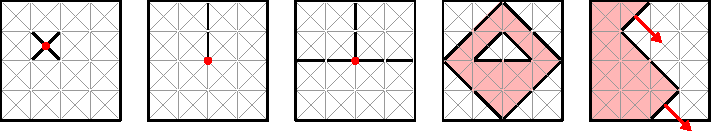
\includegraphics[width=\textwidth]{figs/topology_constraints.pdf}
    \caption{Illustration of the 5 topology constraints (not including symmetry). From left to right: (1) Planarity, no crossing diagonals; (2) No dangling edges; (3) No T-junctions; (4) Full connectivity, no floating polygons; (5) All normals in a polygon must be unique}
\end{figure}


\subsection{Global Topological Constraints}
Once Z3 yields a satisfying assignment based on local constraints, we extract the resulting graph $G=(V,E)$ and pass it through a Python-level global topology filter before accepting it into the database.


\subsubsection{Connectivity Constraint}

First, we require the graph to be a single connected component. Disconnected components represent polygons floating in space within other polygons, which causes severe problems during crease pattern generation. This is easily filtered using NetworkX's built-in connectivity check.

\subsubsection{Unique Normals Constraint}

Second, we validate the internal faces. We utilize a Doubly-Connected Edge List (DCEL) half-edge traversal to extract all faces of the graph: for every vertex $v$, its incident neighbors are sorted angularly using a standard $\text{atan2}(dy, dx)$ function. Walking counter-clockwise around the leftmost turns allows us to systematically extract the closed loops that define the internal polygonal faces.

For each extracted face, we calculate the directional vector 
\[\vec{d} = (\Delta x / \gcd(\Delta x, \Delta y), \Delta y / \gcd(\Delta x, \Delta y))\]
of every boundary segment. We strictly enforce that a valid topological face must consist of sides with unique directions (ignoring sequential collinear segments). While this allows concave polygons, it limits the number of sides to 8 and ensures they do not zig-zag or ``gerrymander'', which would also make crease pattern generation significantly more difficult.

With these local boolean constraints and global topology filters, the SAT solver is able to enumerate all valid topologies.


% =================================
% =================================
% =================================


\section{Database Generation Phase II: Metric Tiling Realization}

The output of the topology enumeration phase is an unweighted planar graph. Although the vertices are temporarily built on an integer grid to guarantee 45$^\circ$ angled edges, the actual locations of the vertices need to be fully constrained to optimize for human-foldability of the crease pattern. This is, after all, the original purpose of 22.5$^\circ$ crease patterns over ``easier'' design methods.

If a topology contains $n$ nodes, we theoretically possess $2n$ degrees of freedom in the Euclidean plane (moving each node in $x$ and $y$). Our objective is to apply constraints until all degrees of freedom are removed, and the tiling is fully locked into a single crease pattern with fully defined references.

\subsection{Basic Geometric Constraints}\label{sec:basic_constraints}
We begin by establishing the absolute requirements of the tiling. We first remove redundant degree-2 vertices from the topology. 

\subsubsection{Angle preservation constraints}
Every edge in the initial grid topology is aligned to a multiple of 45$^\circ$. As the vertices move to form the exact tiling, these edges must remain parallel to their original orientations. Let $\vec{u}$ and $\vec{v}$ be the position of two vertices connected by an edge, and $\hat{n} = (n_x, n_y)$ be the known normal vector of that edge. We enforce the following angular constraint for every edge:
\begin{equation}
    (\vec{v}-\vec{u}) \perp \hat{n}\implies {\hat{n} \cdot (\vec{v} - \vec{u})} = 0 \implies n_x v_x - n_x u_x + n_y v_y - n_y u_y = 0
\end{equation}
Note that this constraint is linear and homogeneous.

\subsubsection{Boundary conditions}
To prevent rigid-body translation and scaling, the bottom-left node is locked to the $(0,0)$, and the top-right node is locked to $(1,1)$. Note that the latter is an inhomogeneous constraint, which prevents the solver from collapsing all vertex coordinates to 0.

\subsubsection{Symmetry constraints}
If the topology was generated with a symmetry constraint, we apply the corresponding symmetry constraints to the coordinates. For example, for book symmetry across the vertical axis $x = N/2$, every pair of symmetric nodes $u$ and $u^*$ must satisfy:
\begin{equation}
    u_x + u^*_x = 1 \quad \text{and} \quad u_y - u^*_y = 0
\end{equation}
Note that this introduces another inhomogeneous constraint. For diagonal symmetry across $y = x$, every pair of symmetric nodes $u$ and $u^*$ must satisfy:
\begin{equation}
    u_x - u^*_y = 0 \quad \text{and} \quad u_y - u^*_x = 0
\end{equation}

We can then combine these linear constraints into a single matrix form $A\vec{x} = \vec{b}$, where $x = {[x_1, y_1, x_2, y_2, \ldots, x_n, y_n]}^T$ is a vector containing all node coordinates, each row of $A$ corresponds to one of the aforementioned linear constraints, and $\vec{b}$ is a vector of constants (mostly zeros, except for the few inhomogeneous conditions). 


To visualize this system, take for example the constraints imposed on the empty square. The global system $A \vec{x} = \vec{b}$, with both the basic geometric constraints as well as a single quadruplet constraint, takes the following structure:
\begin{figure}[h]
    \centering
    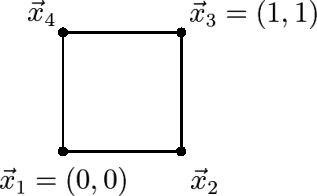
\includegraphics[width=0.3\textwidth]{figs/tiling_square.pdf}
    \caption{Basic geometric constraints on the bare minimum tiling (empty square)}
\end{figure}
\begin{equation}\label{eq:Axb}
\begin{array}{l}
    \text{Edge angle constraints}\\
    \\ \\ \\
    \text{Boundary pinning}\\
    \\ \\ \\
    \text{Diagonal symmetry}\\

    
\end{array}
\underbrace{
    \begin{bmatrix}
        0 & 1 & 0 & -1 & 0 & 0 & 0 & 0\\
        0 &  0 &  1 &   0 & -1  &  0 & 0  & 0  \\
        0 & 0 &  0 &   0 &  0 &  1 &  0 &  -1 \\
        1 &  0 &  0 &  0  &  0 & 0  & -1  & 0  \\
        \hdashline
        1 & 0 & 0 & 0 & 0 & 0 & 0 & 0\\
        0 & 1 & 0 & 0 & 0 & 0 & 0 & 0\\
        0 & 0 & 0 & 0 & 1 & 0 & 0 & 0\\
        0 & 0 & 0 & 0 & 0 & 1 & 0 & 0\\
        \hdashline
        1 & -1 & 0 & 0 & 0 & 0 & 0 & 0\\
        0 & 0 & 0 & 0 & 1 & -1 & 0 & 0\\
        0 & 0 & 1 & 0 & 0 & 0 & 0 & -1\\
        0 & 0 & 0 & 1 & 0 & 0 & -1 & 0\\
        % -1 & 1 & 0 & 0 & 1 &-1 & 0 & 0  
    \end{bmatrix}
}_{A}
\underbrace{
    \begin{bmatrix}
        x_1 \\
        y_1 \\
        x_2 \\
        y_2 \\
        x_3 \\
        y_3 \\
        x_4 \\
        y_4 \\
    \end{bmatrix}
}_{\vec{x}}
=
\underbrace{
    \begin{bmatrix}
        0 \\
        0 \\
        0 \\
        0 \\
        \hdashline
        0 \\
        0 \\ 
        1 \\ 
        1 \\ 
        \hdashline
        0 \\ 
        0 \\
        0 \\ 
        0 \\
        % 0 
    \end{bmatrix}
}_{\vec{b}}
\end{equation}

The crease pattern is fully defined if and only if the matrix $A$ has full rank, $\text{rank}(A) = 2n$. If the matrix is rank-deficient, then there are still degrees of freedom for vertices in the tiling to move without violating constraints. These motions are described by columns of the null space. To resolve these degrees of freedom, we need to inject additional constraints.

\subsection{Quadruplet equidistance constraints}
While only the basic geometric constraints are absolutely necessary, we can ``spend'' the remaining degrees of freedom to constrain the tiling into a crease pattern that is as ``nice'' as possible. It is difficult to quantify how ``nice'' a crease pattern is, but a good heuristic is to minimize the number of internal vertices generated by the straight skeletons of the polygons. This is because internal vertices of a straight skeleton are generally not flat foldable, so each internal vertex forces a propagation of creases that make the crease pattern increasingly messier.

Internal vertices in a straight skeleton appear where 3 or more edges are equidistant from a common point. We can ``collapse'' internal vertices together by forcing $> 3$ sides to be equidistant from a common point. Therefore, we define a \textbf{quadruplet} as a set of 4 edges (not necessarily contiguous) on a polygon, which we can constraint to be equidistant from a shared incircle.

Let $\hat{n}_1, \hat{n}_2, \hat{n}_3, \hat{n}_4$ be the inward-facing unit normal vectors of the four edges in the quadruplet. Let $\vec{v}_1, \vec{v}_2, \vec{v}_3, \vec{v}_4$ be the coordinates of one of the two vertices on each edge. Let $\vec{p} = (p_x, p_y)$ and $r$ be the unknown position and radius of the shared incircle.

For the incircle to be tangent to all four edges simultaneously, the perpendicular distance from the center $\vec{p}$ to each edge $i$ must be exactly equal to $r$. Using vector projection, we can express the distance to a line as:
\begin{equation}
    \hat{n}_i \cdot (\vec{p} - \vec{v}_i) = r \quad \text{for } i \in \{1, 2, 3, 4\}
\end{equation}

We can rearrange this equation to separate the unknown variables ($\vec{p}$ and $r$) from the variables defined by the graph's geometry ($\vec{v}_i$):
\begin{equation}
    \hat{n}_i \cdot \vec{p} - r = \hat{n}_i \cdot \vec{v}_i
\end{equation}

This gives us a system of 4 linear equations. We can represent this system in matrix form as $Q \vec{\xi} = \vec{w}$, where $\vec{\xi}$ contains our unknowns:
\begin{equation}
    \underbrace{
    \begin{bmatrix}
    n_{1x} & n_{1y} & -1 \\
    n_{2x} & n_{2y} & -1 \\
    n_{3x} & n_{3y} & -1 \\
    n_{4x} & n_{4y} & -1
    \end{bmatrix}
    }_{Q}
    \underbrace{
    \begin{bmatrix}
    p_x \\
    p_y \\
    r
    \end{bmatrix}
    }_{\vec{\xi}}
    =
    \underbrace{
    \begin{bmatrix}
    \hat{n}_1 \cdot \vec{v}_1 \\
    \hat{n}_2 \cdot \vec{v}_2 \\
    \hat{n}_3 \cdot \vec{v}_3 \\
    \hat{n}_4 \cdot \vec{v}_4
    \end{bmatrix}
    }_{\vec{w}}
\end{equation}

Notice that $Q$ is a $4 \times 3$ matrix. We have 4 equations but only 3 unknowns ($p_x, p_y$, and $r$). For an overdetermined system to have a valid solution, the right-hand side vector $\vec{w}$ must lie perfectly within the column space of $Q$. We do not actually need to solve for $\vec{\xi}$. We only care that such an incircle exists. If we can eliminate $\vec{\xi}$ entirely, we are left with a relationship that the vertices $\vec{v}_i$ must satisfy.
Recall that a vector $\vec{w}$ is in the column space of $Q$ if and only if it is orthogonal to the left null space of $Q$. Let $\vec{w}^T = \begin{bmatrix} w_1 & w_2 & w_3 & w_4 \end{bmatrix}$ be a basis vector for the left null space of $Q$, such that:
\begin{equation}
    \vec{w}^T Q = \vec{0}^T
\end{equation}
Because the normals $\hat{n}_i$ are strictly fixed constants in the 22.5$^\circ$ system, the matrix $Q$ is constant. Therefore, $\vec{w}$ is also constant and can be precomputed.

For the incircle to exist, we must satisfy:
\begin{equation}
    \vec{w}^T \vec{\xi} = w_1 (\hat{n}_1 \cdot \vec{v}_1) + w_2 (\hat{n}_2 \cdot \vec{v}_2) + w_3 (\hat{n}_3 \cdot \vec{v}_3) + w_4 (\hat{n}_4 \cdot \vec{v}_4) = 0
\end{equation}
By expanding the inner dot products $\hat{n}_i \cdot \vec{v}_i = n_{ix}x_i + n_{iy}y_i$, we group the terms by the coordinate variables of our vertices:
\begin{equation}\label{eq:quadruplet_constraint}
    \sum_{i=1}^{4} \left( (w_i n_{ix}) x_i + (w_i n_{iy}) y_i \right) = 0
\end{equation}
Note that this is a strictly linear, homogeneous constraint acting entirely on the node positions $x_i$ and $y_i$, which can also be expressed as a row in the constraint matrix $A$ without ever solving for the position or radius of the incircle. For example, to add a quadruplet constraint to matrix expanded in Equation~\ref{eq:Axb}, we would append the following row to $A$ and $b$ based on the normals of the rectangle:

\begin{figure}[h]
    \centering
    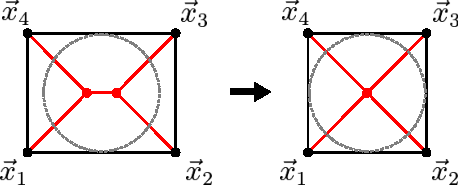
\includegraphics[width=0.5\textwidth]{figs/rectangle_quadruplet.pdf}
    \caption{A rectangular quadruplet constrained to a single equidistant point by Equation~\ref{eq:quadruplet_example}. Note that the constraint in this example is equivalent to asserting that $x_3 - x_1 = y_3 - y_1$, or in other words, the aspect ratio of the rectangle is square.}
\end{figure}

\begin{equation}\label{eq:quadruplet_example}
\begin{bmatrix}
    -1 & 1 & 0 & 0 & 1 &-1 & 0 & 0  
\end{bmatrix}
\begin{bmatrix}
    x_1 \\
    y_1 \\
    x_2 \\
    y_2 \\
    x_3 \\
    y_3 \\
    x_4 \\
    y_4 \\
\end{bmatrix}
=
\begin{bmatrix}
    0 
\end{bmatrix}
\end{equation}


In general, constraining a quadruplet (that contains at least one unconstrained edge) will remove one degree of freedom. However, due to internal symmetries across the tiling, it is possible for a single quadruplet constraint to collapse multiple straight skeleton vertices at once, while still only spending one degree of freedom. Therefore, we want to strategically select quadruplets that maximize the number of straight skeleton vertices they collapse. 

But more importantly, it is possible for a quadruplet constraint to be satisfied but not actually reduce the number of vertices in the straight skeleton. This is because a vertex only appears in the straight skeleton if and only if it is strictly closer to its constituent edges than to any other edge in the polygon. Therefore, if another edge ``invades'' the incircle, the quadruplet constraint is effectively useless. 

Even worse, it is possible for the enforcing of a quadruplet constraint to cause an edge to collapse to 0 or negative length, violating the planarity of the tiling. These two effects are defined by inequalities. Therefore, we must resort to a Mixed-Integer Linear Programming (MILP) formulation to strategically select the optimal set of quadruplets that maximize the number of collapsed straight skeleton vertices while ensuring the physical foldability of the tiling.


\subsection{Quadruplet Harvesting and the MILP Formulator}
To evaluate the physical consequences of activating different quadruplets, the solver must be able to solve the linear system (Equation~\ref{eq:Axb}) for any possible combination of quadruplets, and evaluate the validity of the resulting geometry. Therefore, let the state vector $\vec{X}$ be an augmented version of the vertex coordinate vector $\vec{x}$:
\begin{equation}
    \vec{X} = \left[ \, \vec{x}, \; \vec{z}_{quads}, \; \vec{p}_{incircles}, \; \vec{r}_{incircles}, \; \vec{b}_{bowtie} \, \right]^T
\end{equation}
Where we concatenate the following vectors:
\begin{itemize}
    \item $\vec{x}$: A concatenation of continuous 2D coordinates $\vec{x}_i = (x_i, y_i)$ for every vertex in the graph
    \item $\vec{z}_{quads}$: Boolean decision variables $z_k \in \{0, 1\}$ denoting whether quadruplet candidate $k$ is enforced.
    \item $\vec{p}_{incircles}$: Continuous 2D coordinates $\vec{p}_k = (p_{k_x}, p_{k_y})$ representing the prospective incircle center for quadruplet candidate $k$.
    \item $\vec{r}_{incircles}$: Continuous variables $r_k \ge 0$ representing the prospective incircle radius for quadruplet candidate $k$.
    \item $\vec{b}_{bowtie}$: Boolean variables used to check topological validity of concave polygons.
\end{itemize}

Now recall that the standard form of a MILP problem is:
\begin{align}
    \max_{\vec{X}} \quad & \vec{c}^T \vec{X} \\
    \text{subject to} \quad & M \vec{X} \le \vec{B}
\end{align}
where $\vec{c}$ is the objective function as reward weights on the elements of $\vec{X}$, $M$ is the constraint matrix that encodes all of the linear equalities and inequalities, and $\vec{B}$ stores the constants on the right-hand side of each constraints.


Our objective is to maximize the number of quadruplets that can be activated without violating geometric constraints. Therefore, $\vec{c}$ contains non-zero weights only for the decision variables $\vec{z}_{quads}$. We heavily reward resolving concave (reflex) vertices because they create disproportionately messier crease patterns if not collapsed into a clean internal vertex. Therefore, quadruplets involving reflex vertices are assigned a priority weight ($c_k = 10.0$), while standard convex quadruplets receive a base weight ($c_k = 1.0$).

\subsubsection{Formulating the Constraint Rows}

\paragraph{1. Basic geometric constraints}
First, the same basic geometric constraints described in Section~\ref{sec:basic_constraints} are applied to the vertex coordinates. These constraints only depend on the vertex coordinates $\vec{x}$. These are the only equality constraints (which can be expressed as two inequalities, or sometimes written as a separate matrix).

\paragraph{2. Edge Integrity:}
To prevent edges from collapsing to zero or negative length (inversion), we enforce a minimum feature size, $\epsilon$. Let $\hat{t}$ be the unit tangent vector of an edge. For any directed edge from vertex $\vec{u}$ to vertex $\vec{v}$, the projected distance must remain at least $\epsilon$:
\begin{equation}
    \hat{t} \cdot (\vec{v}-\vec{u}) \ge \epsilon \quad \implies \quad - \hat{t}^T \vec{v} + \hat{t}^T \vec{u} \le -\epsilon
\end{equation}
Note that $\epsilon$ is not for numerical stability, but another metric of crease patern ``niceness''. If $\epsilon$ is too small, the resulting crease pattern may contain tiny creases that are unpleasant to fold. If $\epsilon$ is too large, the solver may not be able to find any valid solutions. We empirically set $\epsilon = \frac{1}{4N}$, where $N$ is the grid size of the original topology.

\paragraph{3. Quadruplet Activation (Big-M Method):}
If $z_k = 1$, quadruplet $k$ must be constrained such that the distance from the incircle center $\vec{P}_k$ to the boundary edge originating at vertex $\vec{u}$ with inward normal $\hat{n}$ must exactly equal the radius $r_k$. However, if $z_k = 0$, we need the constraint to be relaxed. To encode this as linear rows in $M$, we choose a large constant $C\approx 3N$ and apply the following inequalities to a vertex $\vec{u}$ on each edge in the quadruplet:
\begin{align}
    \hat{n}_u^T \vec{p}_k - \hat{n}_u^T \vec{u} - r_k + C z_k \le C \\
    -\hat{n}_u^T \vec{p}_k + \hat{n}_u^T \vec{u} + r_k + C z_k \le C
\end{align}

\paragraph{4. Incircle invasion:}
Recall that a vertex only appears in the straight skeleton if and only if it is strictly closer to its constituent edges than to any other edge in the polygon. Therefore, if another edge ``invades'' the incircle, the quadruplet constraint is effectively useless. To prevent this, we must ensure that any invader edge $i$ maintains a normal projection distance from the incircle center $\vec{P}_k$ that is at least $r_k$:

\begin{equation}
    -\vec{n}_i^T \vec{p}_k + \vec{n}_i^T \vec{x}_i - r_k + C z_k \le C
\end{equation}
The addition of this constraint is why the MILP formulation requires $\vec{p}_k, r_k$ as state variables, while Equation~\ref{eq:quadruplet_constraint} did not.

\begin{figure}[h]
    \centering
    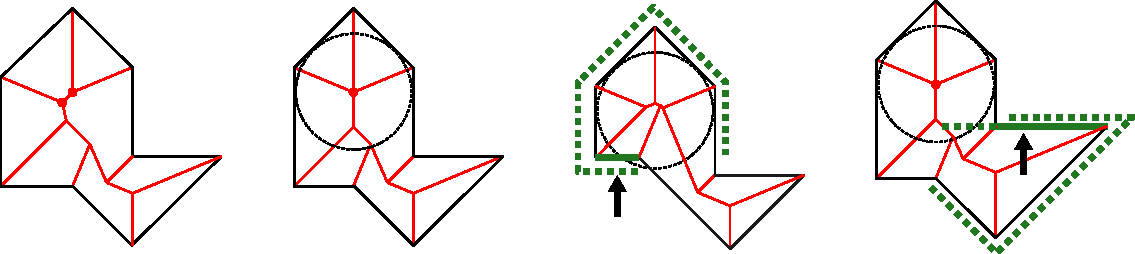
\includegraphics[width=\textwidth]{figs/incircle_invasion.pdf}
    \caption{From left to right: (1) An unconstrained polygon and its messy straight skeleton. (2) Applying an incircle constraint to a quadruplet collapses two interior points into one. (3) If an edge from the same convex chain invades the incircle, the constraint is useless and the straight skeleton is broken. (4) An edge from a different convex chain (separated by a concave vertex) has a normal projection that invades the incircle, but without breaking the straight skeleton.}
\end{figure}

However, this equation treats every side of the polygon as an infinite line, while incircle invasion only occurs if the actual line segment invades the circle. Formulating this stronger constraint woould introduce a quadratic term (Euclidean distance from the incircle center). Therefore, we realize that edges that do not share a convex chain with any edge in the quadruplet are incapable of actually invading the incircle, and as a conservative heuristic, only apply the infinite line incircle invasion constraint to all other edges.

\paragraph{5. Anti-Bowtie Clearance:}
In some concave polygons, it is possible for a concave ``mouth'' vertex to clip through an edge on the opposite side of the polygon.

For every reflex vertex $\vec{x}_c$ and a non-adjacent edge $(\vec{u}, \vec{v})$ with normal $\hat{n}$ and tangent $\hat{t}$, we create three boolean variables based on the vertex's position relative to the edge: 
\begin{itemize}
    \item $b_1$ = 1 if $\hat{n} \cdot (\vec{x}_c - \vec{u}) < 0$ (the vertex is behind the edge)
    \item $b_2$ = 1 if $\hat{t} \cdot (\vec{x}_c - \vec{u}) > 0$ (the vertex is to the left of the edge)
    \item $b_3$ = 1 if $\hat{t} \cdot (\vec{x}_c - \vec{u}) < 0$ (the vertex is to the right of the edge)
\end{itemize} 

\begin{figure}[h]
    \centering
    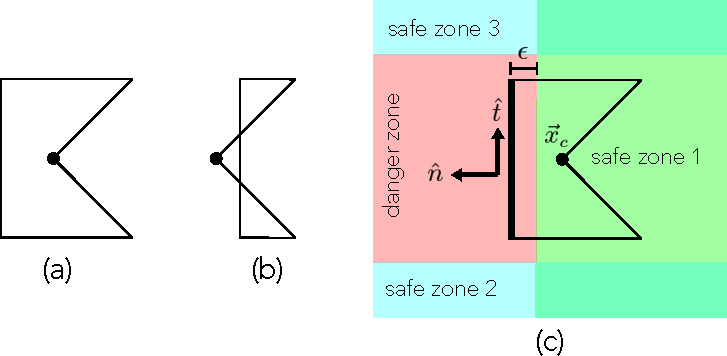
\includegraphics[width=0.6\textwidth]{figs/bowtie.pdf}
    \caption{Left: an unconstrained polygon. Center: the polygon with a ``bowtie'' violation. Right: the three safe zones defined by $b_1,b_2,b_3$ and the danger zone (red) where the constraint is violated, defined by the edge's vectors $\hat{n},\hat{t}$ and minimum clearance size $\epsilon$.}
\end{figure}


We can enforce that the reflex vertex must reside in at least one safe sector by applying the constraint:
\[b_1 + b_2 + b_3 \ge 1 \implies -b_1 - b_2 - b_3 \le -1\]
The MILP solver gets to choose which of $b_1, b_2, b_3$ is true. Similar to the quadruplet toggles $z_k$, we can use big-M constraints to link these boolean variables to toggle which which safe zone the vertex is constrained to. For example, the corresponding constraint for $b_1$ would be:
\begin{equation}
    \hat{n} \cdot (\vec{x}_c - \vec{u}) \ge \epsilon - C(1 - b_1) \quad \implies \quad -\hat{n}^T \vec{x}_c + \hat{n}^T \vec{u} + C b_1 \le C - \epsilon
\end{equation}
Recall that these constraints are added for every pair of reflex vertex and non-adjacent edge. 

\subsubsection{The Compound Matrix Inequality}
By concatenating these varied constraints, we construct the master MILP matrix equation. The inequality system $M \vec{X} \le \vec{B}$ takes the following block matrix structure:\footnote{Technically, the basic geometric constraints should be in a separate matrix because they represent equalities rather than inequalities, though for the sake of visual compactness we can handwave that each equality can be represented as a pair of inequalities.}

\begin{equation}\label{eq:milp}
\begin{array}{l}
    \text{Basic constraints} \\
    \text{Edge Integrity} \\
    \text{Quadruplets} \\
    \\
    \text{Incircle Clearance} \\
    \\
    \text{Anti-bowtie}
    \\
\end{array}
\underbrace{
\left[
\begin{array}{ccccc}
    A & 0 & 0 & 0 & 0 \\
    \hdashline
    M_{edges} & 0 & 0 & 0 & 0 \\
    \hdashline
    -N_{quad} & C \cdot I_{quad} & N_{incircle} & -I_{quad} & 0 \\
    N_{quad} & C \cdot I_{quad} & -N_{incircle} & I_{quad} & 0 \\
    \hdashline
    N_{invader} & C \cdot I_{inv} & -N_{incircle} & -I_{inv} & 0 \\
    \hdashline
    0 & 0 & 0 & 0 & -S_{sector} \\
    N_{bowtie} & 0 & 0 & 0 & C \cdot I_{bowtie} 
\end{array}
\right]}_{M}
\underbrace{
\begin{bmatrix}
    \vec{x} \\
    \vec{z}_{quads} \\
    \vec{P}_{incircles} \\
    \vec{r}_{incircles} \\
    \vec{b}_{bowtie}
\end{bmatrix}}_{\vec{X}}
\le
\underbrace{
\begin{bmatrix}
    \mathbf{0} \\
    \hdashline
    -\boldsymbol{\epsilon} \\
    \hdashline
    \mathbf{C} \\
    \mathbf{C} \\
    \hdashline
    \mathbf{C} \\
    \hdashline
    -\mathbf{1} \\
    \mathbf{C} - \boldsymbol{\epsilon}
\end{bmatrix}}_{\vec{B}}
\end{equation}

Where:
\begin{itemize}
    \item $M_{edges}$ applies the tangent vector projections ($\hat{t}^T$) mapping adjacent vertices to their required edge clearance.
    \item $N_{quad}$, $N_{invader}$, and $N_{bowtie}$ apply the corresponding inward normal and tangent projections ($\hat{n}^T, \hat{t}^T$) mapping vertices to their respective distance inequalities.
    \item $N_{incircle}$ projects the prospective incircle centers ($\vec{P}_k$) against those same normal vectors.
    \item $S_{sector}$ is a block summation matrix that groups and adds the three boolean sector variables $(b_1 + b_2 + b_3)$ for each reflex-edge pair.
    \item $I$ represents identity matrices of the appropriate dimensions mapping the scalar variables ($\vec{r}_{incircles}$ and the boolean toggles).
    \item $\mathbf{C}$, $\boldsymbol{\epsilon}$, and $\mathbf{1}$ represent column vectors populated dynamically with the respective constants.
\end{itemize}
In total, $M$ and $\vec{B}$ are composed of pre-computable constants for each topology. The problem in this form can be passed into a MILP solver like PuLP to constrain the maximum number of quadruplets while maintaining the geometric validity of the tiling.

\subsubsection{Iterative Integer Cuts for Database Diversity}
A single topology can often be tiled in several geometrically distinct ways. To populate the database with diverse layouts from the same root topology, we loop the MILP solver. Upon finding an optimal set of active quadruplets $\mathcal{A}$, we log the configuration and inject a strict integer cut back into the solver:
\begin{equation}
    \sum_{i \in \mathcal{A}} z_i \le |\mathcal{A}| - d_{threshold}
\end{equation}
where $d_{threshold}$ is a hyperparameter defining the minimum diversity difference between solutions. This bans the previous solution and forces the MILP to swap at least $d_{threshold}$ quadruplets, nudging it to discover alternative geometric variations---though it is not guaranteed that the resulting tilings will be unique, even if the sets of selected quadruplets are different.

%% TODO in the section above: be consistent between v and x. probably use v for vertex coordinates

\subsection{Quadruplet harvesting}

The solution to the MILP comes with a set of vertex positions that is guaranteed to be physically realizable (satisfying the constraints applied to $M$). However, it cannot guarantee that the tiling is fully locked. This is because it is computationally prohibitive to feed every possible quadruplet into the MILP (consider the fact that an $n$-gon contains $\binom{n}{4}$ possible quadruplets), so we initialize it with a heuristic ``harvest'' of quadruplets that are either contiguous or are the nearest edges to a concave pair of edges. As a result, the MILP might overlook a key quadruplet needed to fully constrain the tiling.

Before performing the expensive Gauss-Jordan elimination, we check the algebraic rank of the constraint matrix $M$. To do this instantaneously, we perform Gaussian Elimination over a finite field $Z_p$ using a large prime (e.g., $P = 1000000007$). 

If the matrix is rank-deficient, the $Z_p$ elimination identifies exactly which columns (variables) lack pivots. We map these free variables back to their physical nodes, identifying the "sliding nodes." We then initialize a \textbf{Directed Depth-First Search (DFS) Scavenger}. The DFS explores the pool of unused, exhaustive quadruplet candidates, specifically filtering for quadruplets that involve the identified sliding nodes. It tentatively adds their 4D nullspace equations to $M$ and re-evaluates the rank. Once the matrix achieves full rank (exactly $4n$), the DFS terminates.

Finally, the full-rank constraint matrix is passed to our custom C++ \texttt{Fraction} class routines, which execute exact Gauss-Jordan elimination to solve for the absolute 4D coordinates of the metric tiling.


This process is thorough, albeit roundabout. First we use heuristics to choose which quadruplets to consider first. Then we use MILP to select which of those quadruplets are the best, by applying constraints to the constraints themselves. If it turns out that the MILP selection is not sufficient, we have to go back and scavenge through the unconsidered quadruplets to find which quadruplets would make $A$ full rank. Only then do we actually apply the quadruplet constraints and solve for the vertex coordinates.


\subsection{The Exact Linear Solver and the Two-Row Formulation}
The MILP provides a guaranteed-safe set of geometric intents, but floating-point MILP coordinates are too noisy for strict origami raycasting. We must lock these intents into an exact fractional matrix in the 4D Hypercube basis $\mathbb{Q}^4$. 

Consider a standard angular constraint requiring the edge between node $u$ and node $v$ to remain parallel to a known 22.5$^\circ$ directional vector $\vec{d} = (d_x, d_y)$. The 2D cross product must be exactly zero:
\begin{equation}
    (v_x - u_x)d_y - (v_y - u_y)d_x = 0
\end{equation}
In our 4D basis, the physical 2D coordinates are derived from the 4D rational coordinates: $u = [x_1, y_1, z_1, w_1]^T$ and $v = [x_2, y_2, z_2, w_2]^T$. Substituting the hypercube projection mapping:
\begin{align}
    \Delta X &= (x_2 - x_1) + \frac{\sqrt{2}}{2}((y_2-y_1) - (w_2-w_1)) = A_x + B_x \sqrt{2} \\
    \Delta Y &= (z_2 - z_1) + \frac{\sqrt{2}}{2}((y_2-y_1) + (w_2-w_1)) = A_y + B_y \sqrt{2}
\end{align}
The directional vector $\vec{d}$ is similarly defined as $d_x = a_x + b_x \sqrt{2}$ and $d_y = a_y + b_y \sqrt{2}$. Substituting these components into the cross product yields a polynomial expansion:
\begin{equation}
    (A_x + B_x \sqrt{2})(a_y + b_y \sqrt{2}) - (A_y + B_y \sqrt{2})(a_x + b_x \sqrt{2}) = 0
\end{equation}
When the algebra is expanded and simplified, the variables naturally separate into two groups: those multiplied by 1, and those multiplied by $\sqrt{2}$. It takes the form:
\begin{equation}
    C_{rational} + C_{irrational} \sqrt{2} = 0
\end{equation}
Crucially, because $\sqrt{2}$ is an irrational number, it is impossible for a non-zero rational number to cancel out a non-zero irrational number. Therefore, for the physical angle to be exactly zero, \textbf{both coefficients must independently evaluate to exactly zero}. 

This is the core insight of the SEARCH 22.5 exact solver architecture: \textbf{Every single physical 2D geometric constraint generates exactly two independent rows in the 4D algebraic constraint matrix.}
\begin{align}
    \text{Row 1:} \quad & C_{rational}(x_1, y_1, z_1, w_1, x_2, y_2, z_2, w_2) = 0 \\
    \text{Row 2:} \quad & C_{irrational}(x_1, y_1, z_1, w_1, x_2, y_2, z_2, w_2) = 0
\end{align}

\textcolor{red}{[Figure Placeholder: A visual matrix diagram showing the $Ax=b$ formulation. On the left, display a graph with a single highlighted edge. On the right, display the constraint matrix, explicitly showing how the $x, y, z, w$ columns of nodes $u$ and $v$ populate two distinct rows for that single physical edge.]}


\section{Database Generation Phase III: Crease Patterns and Folding}

The exact tiling establishes a flawless 4D geometric foundation, locking the perimeter and the major structural nodes of the base. However, this abstract metric graph must now be routed into a physically flat-foldable Crease Pattern (CP) and subsequently folded into a layered 2D state to extract its structural tree.

\subsection{The Float-to-Exact Straight Skeleton}
To route the interior creases of the faces defined by the tiling, we utilize a straight skeleton algorithm. Because native exact-fraction straight skeleton algorithms are computationally prohibitive, we implement a hybrid "Float-to-Exact" mapping architecture. 

First, we project the 4D exact vertices of a face into 2D floating-point Cartesian coordinates. To bypass the well-documented IEEE-754 singularity failures inherent to standard floating-point sweep-line algorithms, we apply an aggressive quantization filter, truncating coordinates to a fixed precision (\texttt{QUANTIZATION\_DECIMALS = 3}) and deduplicating antiparallel spikes created by the MILP's vertex collapsing.

We feed this sanitized floating-point polygon into an off-the-shelf straight skeleton library to extract the \textit{topological connectivity} of the interior creases. To reclaim exact mathematical precision, we map these floating-point nodes back to the $\mathbb{Q}^4$ hypercube grid. 
For boundary nodes, we search the exact 4D coordinate dictionary using a tight capture radius (\texttt{SNAP\_TOLERANCE = 1e-3}). For internal nodes, we iteratively look at their resolved neighbors, extract the 22.5$^\circ$ directional angles of the incident creases, and perform an exact 4D algebraic intersection. This hybrid approach grants us the extreme speed of floating-point topological algorithms while guaranteeing the 100\% rational geometric perfection of the final vertices.

\subsection{Kawasaki Propagation and Hinge Routing}
The resulting straight skeleton routes the paper efficiently, but it makes no guarantees regarding flat-foldability. In origami, Kawasaki's Theorem mandates that for a vertex to fold flat, the alternating sum of the angles between its incident creases must equal exactly $180^\circ$ (or an alternating sum of 8, in our 22.5$^\circ$ integer units).

We observe that the straight skeleton inherently creates degree-3 vertices (which trivially violate Kawasaki's theorem) and other odd-degree intersections. To enforce flat-foldability, we developed a greedy Kawasaki-fixing algorithm utilizing recursive 4D raycasting.

The algorithm filters for odd-degree vertices that violate Kawasaki. For a target vertex, it evaluates two primary strategies:
\begin{enumerate}
    \item \textbf{Hinge Addition:} It tentatively casts an auxiliary "hinge" ray outward along all 8 valid 22.5$^\circ$ directions. 
    \item \textbf{Hinge Removal:} It tentatively removes an existing hinge and recursively collapses any adjacent degree-3 vertices that are subsequently rendered redundant.
\end{enumerate}
When a hinge ray is cast into a polygonal face, physical logic dictates it can only intersect the bounding edges of that specific face. We calculate the exact 4D intersection; if the ray strikes a boundary crease, it splits the edge, generates a new vertex, and reflects perfectly across the crease to propagate into the adjacent face.

Because one added hinge can cascade across the entire paper, we execute these tests on ultra-fast, shallow-copied clones of the CP. We evaluate each transformation using a strict cost metric: \texttt{(Remaining Odd Kawasaki Errors, Total Operations/Hinges Added)}. The algorithm permanently commits the transformation that resolves the local angular defect while minimizing the addition of new, cluttering creases. 

\textcolor{red}{[Figure Placeholder: A sequential diagram of Kawasaki Propagation. Frame 1: A degree-3 vertex in a straight skeleton. Frame 2: An auxiliary hinge ray is cast, splitting a neighboring edge. Frame 3: The ray reflects and propagates until it terminates at a boundary, leaving a fully valid, even-degree crease mesh.]}

\subsection{The Stacked Folded State Architecture}
Once the CP is strictly valid, we algorithmically fold it into a mathematically flat 2D state. The CP explicitly tracks topological faces via Doubly-Connected Edge List (DCEL) logic, sorting half-edges counter-clockwise and discarding the infinite outer face using signed-area calculations . 

To calculate the 2D folded coordinates, we construct a spanning tree of the faces via a Kinematics Breadth-First Search (BFS). Starting from an arbitrary root face, we walk the adjacency graph, recursively reflecting the exact 4D vertices of child faces across their connecting hinge edges.

However, calculating coordinates alone is insufficient; we must track the physical layering of the paper. We define a highly specialized data structure, \texttt{Fold225}, which separates abstract topological faces from physical paper layers (\textit{instances}):
\begin{itemize}
    \item \texttt{vertices}, \texttt{edges}, \texttt{faces}: The core geometric definitions in the folded 2D plane.
    \item \texttt{instances}: A list of stacks. Stack $f$ corresponds to face $f$. If a face folds back onto itself multiple times, its stack will contain multiple \textit{instances}.
\end{itemize}
Every instance possesses an implied address $(f, i)$, where $f$ is the face index and $i$ is its depth in the stack. Within the stack, an instance is represented solely by its connections to other instances across its perimeter edges. For example, if instance $(f_1, i_1)$ connects across edge $e$ to instance $(f_2, i_2)$, that address is logged in its connection array. Boundary edges simply terminate in a \texttt{Null} pointer. This pointer-based architecture completely models the non-manifold, layered reality of folded paper.

\subsection{Orthogonal Slicing and Tree Extraction}
With the paper successfully folded into a layered stack of 2D polygons, we must extract its uniaxial "Stick Figure" (the macroscopic tree). Because all layers overlap, we execute an orthogonal slicing algorithm---conceptually identical to a medical CT scan---to isolate the connected appendages.

First, we determine the optimal projection axis $\vec{a}$ by evaluating the bounding box width along the primary orthogonal and diagonal vectors, selecting the axis that yields the maximum span. Every vertex $\vec{v}_i$ in the folded state projects a critical height onto this axis: $h_i = \vec{v}_i \cdot \vec{a}$. We isolate and sort the unique critical heights generated by the vertices .

We mathematically sweep a 1D slice line $\mathcal{L}(h)$ perpendicular to $\vec{a}$. Between any two adjacent critical heights $(h_i, h_{i+1})$, the topology of the folded layers is entirely immutable. Therefore, we sample the structure precisely at these critical heights.

When a slice intersects the folded state, it severs the topological faces. We utilize a highly optimized C++ routine (\texttt{split\_and\_rebuild\_cpp}) to bifurcate the affected faces and instantly remap the multi-layered instance pointers to the newly severed geometry. 

To extract the tree, we build an adjacency graph of the instances. Crucially, \textbf{we ignore any connections that occur across edges parallel to the slicing hinge} . By filtering these out, the instances cluster into discrete Connected Components, representing the physical "flaps" or "rivers" of the origami base flowing between the critical height slices. 

Every connected component spanning between two slices forms an \textbf{Edge} in our macroscopic tree, with its length directly proportional to the physical axial distance $h_{i+1} - h_i$. Where these components converge and physically interact at a critical height slice, they form a \textbf{Node} in the tree. By collapsing and merging intermediate degree-2 nodes, the microscopic complexity of overlapping paper layers is flawlessly distilled into an abstract, undirected graph representing the physical appendages of the origami model  .

\textcolor{red}{[Figure Placeholder: The Slicing Algorithm. Show a folded base on the left with a 1D projection axis. In the center, show exploded views of the physical instance layers at three different slice heights. On the right, show the final extracted graph tree, visually mapping edges of the graph to the connected components (flaps) of the layers.]}
\section{Database Architecture and Infrastructure}
To manage the generation of millions of crease patterns and their high-dimensional representations, SEARCH 22.5 implements a decoupled, highly parallelized database architecture utilizing SQLite, SQLAlchemy, and Python's \texttt{multiprocessing} library. The generation pipeline is strictly separated into two independent databases: the Topologies database and the Tilings database.

\subsection{Phase I Storage: Topology Database}
The Topology database (\texttt{topologies\_N\_symmetry.db}) acts as the initial repository for the Z3 SAT solver outputs. To manage the parallel workload efficiently, a \texttt{Prefix} table acts as a task queue, tracking which binary prefixes have been fully exhausted by the worker processes.

When a worker discovers a valid topology, the configuration of its internal edges is serialized into a highly compressed bit-string. To ensure uniqueness and provide a rapid indexing mechanism, this bit-string is hashed into a 64-bit integer using MurmurHash3 (\texttt{mmh3}). The topology is saved to the \texttt{State} table using a native \texttt{INSERT ... ON CONFLICT DO NOTHING} command. By shifting the deduplication burden down to the SQLite C-engine via the \texttt{hashed\_state} index, the Python worker processes can asynchronously write thousands of states per second without encountering race conditions or requiring expensive cross-process locking locks.

\subsection{Phase II Storage: Tiling Database}
The Tiling database (\texttt{tilings\_N\_symmetry.db}) is populated by an orchestrator script that pulls pending topologies from Phase I. Because the MILP quadruplet solver can generate multiple geometrically distinct tilings from a single topology via our diversity integer cuts, the Tiling database implements a one-to-many schema .

For each valid metric tiling successfully generated, canonicalized, and flat-folded, three key data structures are stored:
\begin{enumerate}
    \item \texttt{hashed\_tiling}: A 64-bit MurmurHash3 integer derived from the canonicalized exact 4D coordinate geometry. This prevents identically routed straight skeletons (which can occasionally emerge from different MILP branches) from duplicating in the database.
    \item \texttt{tiling\_blob}: A fully serialized (Pickled) dictionary containing the exact $\mathbb{Q}^4$ vertices, the exact edge connectivity, and the topological faces, allowing the crease pattern to be perfectly reconstructed downstream.
    \item \texttt{embedding}: A dense 32-dimensional NumPy array (\texttt{float32} bytes) representing the tree's spectral fingerprint, optimizing the memory footprint for machine learning similarity searches.
\end{enumerate}

\section{Spectral Graph Theory and Tree Embedding}

To map the extracted uniaxial stick-figure trees into a searchable continuous vector space, SEARCH 22.5 leverages Spectral Graph Theory. 

\subsection{Literature Review: The Graph Laplacian}
Spectral graph theory analyzes the properties of a graph in relationship to the characteristic polynomial, eigenvalues, and eigenvectors of matrices associated with the graph, most notably the Adjacency matrix $A$ and the Laplacian matrix $L$ \cite{chung1997spectral}. The Laplacian is defined as $L = D - A$, where $D$ is the diagonal degree matrix.

The Laplacian matrix has been shown to hold immense representational power for graph topologies. Because $L$ is a symmetric, positive semi-definite matrix, its eigenvalues are real and non-negative: $0 = \lambda_1 \le \lambda_2 \le \dots \le \lambda_n$. The multiplicity of the zero eigenvalue corresponds exactly to the number of connected components in the graph. For a connected graph (like an origami tree), $\lambda_1 = 0$ and $\lambda_2 > 0$. 

This second smallest eigenvalue, $\lambda_2$, is famously known as the \textit{algebraic connectivity} or the \textit{Fiedler value}, introduced by Miroslav Fiedler in 1973 \cite{fiedler1973algebraic}. The Fiedler value dictates the global connectivity and structural bottlenecks of the network. Furthermore, eigendecompositions of the Laplacian have been extensively and successfully utilized in computer vision and geometric hashing for graph-matching problems, as isomorphic graphs are strictly cospectral (sharing identical eigenvalues), while the Laplacian spectrum provides robust, graded continuous distances for non-isomorphic but structurally similar shapes \cite{de2007old}. 

\subsection{The 32-Dimensional Fingerprint}
Following this theoretical precedent, we compute the eigenvalues of the Laplacian matrix $L$ for every extracted origami tree. The edge lengths of the tree (derived from the orthogonal slicing heights) are mapped to graph weights $w_{uv} = 1 / L_{uv}$, such that short, tight flaps exhibit stronger algebraic connectivity bounds than long, sweeping branches  .

The eigenvalues are calculated via standard numerical linear algebra (\texttt{np.linalg.eigvalsh}). Because all valid origami bases exist as a single connected component, the trivial $\lambda_1 = 0$ eigenvalue is systematically discarded. The remaining non-zero eigenvalues are sorted in ascending order. To ensure the database maintains a uniform mathematical dimensionality regardless of the complexity of the origami base, the sequence is either truncated or padded with trailing zeros to exactly 32 dimensions (\texttt{DIMENSION = 32})  . This 32-dimensional continuous vector serves as the immutable geometric fingerprint for the database.

\section{Database Querying and Retrieval}
The ultimate objective of SEARCH 22.5 is to allow a user to retrieve a complex, exact-fraction crease pattern in constant time. This is achieved via our Query Pipeline and the interactive graphical interface.

\subsection{Ephemeral FAISS Indexing and NumPy Caching}
A standard SQLite database is highly inefficient for high-dimensional vector similarity searches. Furthermore, standard indexing structures are rigid; altering the geometric importance of certain graph features would traditionally require mutating and re-saving the entire multi-gigabyte database.

To bypass this, we maintain a raw \texttt{.npy} (NumPy) cache of the database embeddings alongside an ordered mapping array . Loading a dense matrix directly into RAM from a binary \texttt{.npy} file is over 100 times faster than iterating through SQLite blobs. At query time, the system loads this matrix and constructs an ephemeral FAISS (Facebook AI Similarity Search) \texttt{IndexFlatL2} index entirely in memory. This allows the search algorithm to instantly scan millions of 32-dimensional vectors and retrieve the nearest L2 (Euclidean) matches in mere milliseconds.

\subsection{Eigenvalue Weighting and Tuning}
Raw Euclidean distance across the Laplacian spectrum is flawed for origami design. High eigenvalues ($\lambda \ge 2.0$) correspond to localized, high-frequency structures within the graph, such as minor topological forks or tiny flaps at the tips. Conversely, low eigenvalues ($\lambda \le 0.5$) govern the global, macroscopic branches (the spine, the major appendages). In origami design, matching the global proportions of the base is vastly more important than precisely mirroring the microscopic flaps.

Because our FAISS index is ephemeral, we can apply dynamic scaling weights to both the query vector and the entire database matrix instantaneously at query time . We implemented three distinct weighting architectures:
\begin{itemize}
    \item \textbf{Value Decay:} Weights drop exponentially as the eigenvalue itself increases: $w_i = e^{-t \cdot \lambda_i}$.
    \item \textbf{Index Decay:} Weights drop strictly based on the dimensional sequence order: $w_i = e^{-t \cdot i}$.
    \item \textbf{Inverse:} An aggressive, physics-inspired harmonic penalty: $w_i = 1 / (\lambda_i + \epsilon)$.
\end{itemize}
Empirical testing on thousands of interactive queries demonstrated that \textbf{Value Decay} with a parameter of $t \approx 0.03$ perfectly balances structural fidelity and local flexibility, heavily penalizing mismatches in the global Fiedler values while remaining highly tolerant of extra flaps at the tips of the branches.

\subsection{Interactive GUI}
To bridge the gap between human design and the hyperspace index, we built an interactive Matplotlib GUI. The user is presented with a blank canvas and can click and drag to draw a completely custom uniaxial stick figure . 

The spatial coordinates of the drawn nodes define the Euclidean lengths of the physical flaps. When the query is executed, the GUI constructs a NetworkX graph, normalizes the edge lengths, extracts the Laplacian eigenvalues, applies the $t=0.03$ value decay, and pings the FAISS engine. The result is a unified Megaplot that instantaneously presents the user with the mathematically perfect 22.5$^\circ$ crease patterns whose internal folded skeletons most closely map to their hand-drawn intent.
\section{Computational Scaling and Architecture}
The combinatorial explosion of valid grid topologies represents the primary computational bottleneck. Exhaustive profiling reveals the total number of states $\mathcal{N}(N)$ scales with the area of the grid:
\begin{equation}
    \mathcal{N}(N) \sim \mathcal{O}(\gamma^{N^2})
\end{equation}
Empirical data establishes $\gamma \approx 5.5$. Utilizing Python multiprocessing paired with C++ \texttt{pybind11} bindings, a single state traverses the entire pipeline in approximately 0.4 seconds, requiring 0.04 KB of SQLite storage. While databases up to $N=5$ synthesize effectively on standard workstation clusters, pushing the architecture to $N=6$ and beyond moves directly into the domain of dedicated supercomputing.



\subsection{Parallelization via Prefix Pruning}
As grid area expands, the search space $O(2^{4N^2})$ rapidly exceeds the capacity of a single SAT solver instance. To solve this, we implemented a massive multiprocessing architecture utilizing \textit{prefix seeding}.

The internal edges are given a strict, deterministic ordering. We can divide the search space by hardcoding the first $k$ edges to a specific binary prefix (e.g., `10110...`), leaving the solver to find valid configurations for the remaining $(4N^2 - 2N) - k$ edges. 

However, naively generating all $2^k$ prefixes results in millions of "dead" prefixes that inherently violate the planarity or degree constraints within their first few bits. To solve this efficiently, we execute a \textit{Pre-Pruning Phase}. We spin up a miniature Z3 instance containing only the base geometric rules, and constrain its search exclusively to the first $k$ variables. We iteratively extract valid models, blocking previously found prefixes by adding the logical negation of their exact bit-state back to the solver:
\begin{equation}
    \text{Block Clause} = \bigvee_{i=1}^k (v_i \neq b_i)
\end{equation}
This drastically shrinks the search tree. For example, an 18-bit prefix sequence natively contains 262,144 combinations, but Z3 dynamically pre-prunes this down to merely $\sim$40,000 viable prefixes.

These viable prefixes are stored in a centralized SQLite database queue. Parallel worker processes fetch a prefix, initialize a fresh Z3 solver with the prefix hardcoded as absolute truth, and exhaustively discover every valid topology that exists down that specific branch of the combinatorial tree. 

\subsection{Canonicalization and Database Storage}
Because the SAT solver inherently generates isomorphically identical graphs rotated or reflected across the paper, we canonicalize the geometries before saving. 

We apply all 8 rigid transformations of the $D_4$ group to the active edge set. The edges are strictly sorted, and the transformation that yields the lexicographically smallest edge tuple is selected as the canonical absolute representation of that topology. 

To minimize disk I/O and storage overhead, the canonical edge list is compressed into a contiguous binary byte-string, representing the truth states of the ordered edges. A 64-bit MurmurHash3 (\texttt{mmh3}) integer is generated from this byte-string. The worker flushes these states in batches of 50 to an SQLite writer process, which utilizes a native `INSERT ... ON CONFLICT DO NOTHING` statement bound to the 64-bit hash index. This pushes the deduplication burden down to the C-level of the database engine, rendering it lightning-fast, immune to uncommitted batch duplicates, and highly resilient to process interruptions.


\section{Conclusion}
SEARCH 22.5 fundamentally reframes the computational origami design flow. By shifting the computational burden of integer programming and exact Gaussian elimination to an exhaustive precomputation phase, we enable instantaneous, constant-time design retrieval. The utilization of the 4D Hypercube basis natively prevents floating-point inaccuracies, while our orthogonal slicing and spectral embedding techniques establish a robust bridge between abstract user intent (trees) and exact physical realizations (tiled crease patterns).


database scaling: how big of a database is necessary for good results, and how much training time and database memory size is required

quality of results

\printbibliography


\end{document}